\section{Suche}

Um die Resultate der Suche zu bewerten werden nachfolgend Situationen aufgestellt und die von der Suche
vorgeschlagenen Stösse untersucht.

Die erste Situation ist in Abbildung \ref{fig:search_situation_1} ersichtlich.
Der Spielball ist auf der linken Seite des Tisches und es liegen einige rote Kugeln auf dem Tisch verstreut.
Die Kugeln 1, 2 und 3 sind nahe bei den Löchern unten-links, oben-rechts resp. oben-zentral.
Kugel 4 ist in der Nähe des Spielballs, die Kugel 5 ist nahe dem Tischzenturm aufgestellt.

%
%State (for reproducing the results):
%WHITE1, WHITE, -564.147, 9.06096
%RED2, RED, -47.218, -100.06
%RED4, RED, 2.93182, 398.78
%RED5, RED, -865.047, -388.453
%RED6, RED, -629.728, 87.0048
%RED7, RED, 851.622, 398.78
%
\begin{figure}[h!]
    \begin{center}
        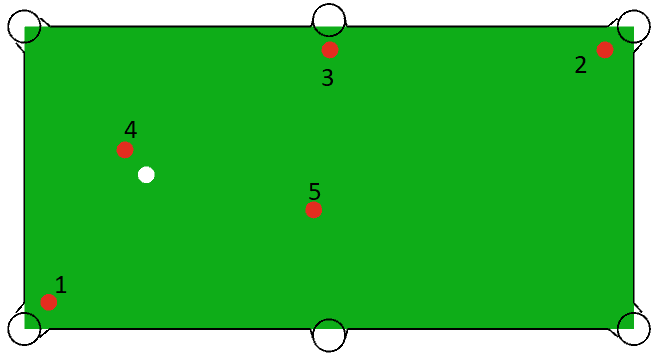
\includegraphics[width=0.4\linewidth]{../common/04_results/resources/simple_search/situation_diverse.PNG}
    \end{center}
    \caption{Situation 1: Einige verstreute Kugeln}
    \label{fig:search_situation_1}
\end{figure}

Nach Betrachten dieser Situation sind einige mögilche Stösse denkbar:
\begin{enumerate}
    \item Kugel 1 ins Loch unten-links.
    \item Kugel 2 ins Loch oben-rechts.
    \item Kugel 3 ins Loch oben-zentral.
    \item Kugel 4 ins Loch oben-links.
    \item Kugel 5 ins Loch unten-rechts.
    \item Kugel 5 ins Loch unten-zentral.
\end{enumerate}

In Abbildung \ref{fig:situation_1_solutions} sind die von der Suche gefundenen Stösse in aufsteigender Schwierigkeit abgebildet.
Mit den ersichtlichen weissen Linien auf jeder Abbildung ist der Pfad jeder Kugel, nicht nur des Spielballs, aufgezeichnet.
Diese voraussichtlichen Pfade werden nach der Suche mithilfe der Simulation des gefundenen Stosses eingezeichnet.

% TODO: bilder ersetzen, sobald die simulation final ist, damit der Pfad der weissen Kugel etwa stimmt.
\begin{figure}
    \centering
    % TODO: in abbildung zu stoss 1 den queue entfernen
    \begin{subfigure}[b]{0.3\textwidth}
        \centering
        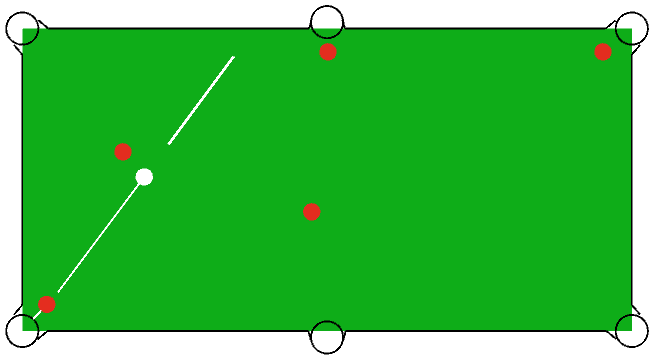
\includegraphics[width=1.0\linewidth]{../common/04_results/resources/simple_search/situation_diverse_solution_1.PNG}
        \caption{Stoss 1}
        \label{fig:situation_1_solution_1}
    \end{subfigure}
    \hfill
    \begin{subfigure}[b]{0.3\textwidth}
        \centering
        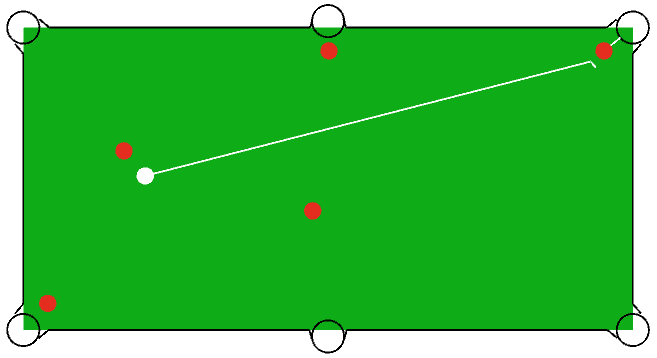
\includegraphics[width=1.0\linewidth]{../common/04_results/resources/simple_search/situation_diverse_solution_2.PNG}
        \caption{Stoss 2}
        \label{fig:situation_1_solution_2}
    \end{subfigure}
    \hfill
    \begin{subfigure}[b]{0.3\textwidth}
        \centering
        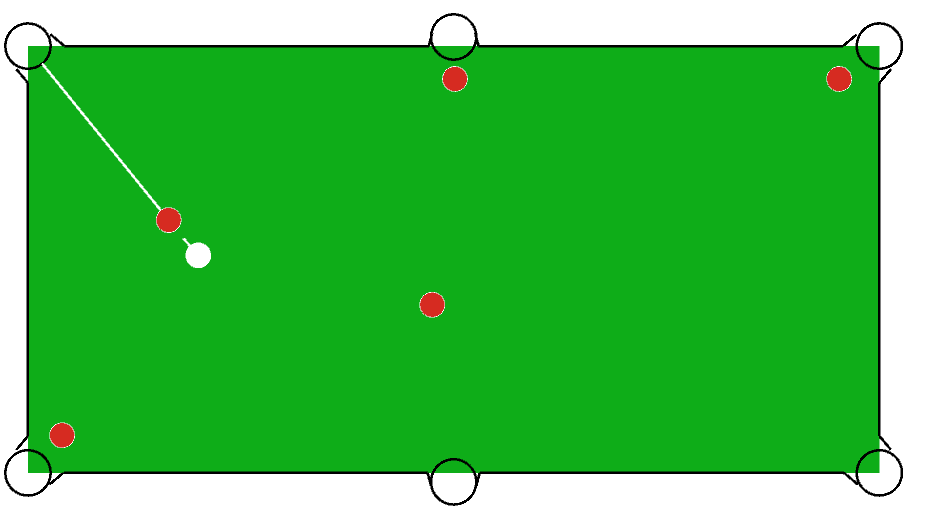
\includegraphics[width=1.0\linewidth]{../common/04_results/resources/simple_search/situation_diverse_solution_3.PNG}
        \caption{Stoss 3}
        \label{fig:situation_1_solution_3}
    \end{subfigure}
    \begin{subfigure}[b]{0.3\textwidth}
        \centering
        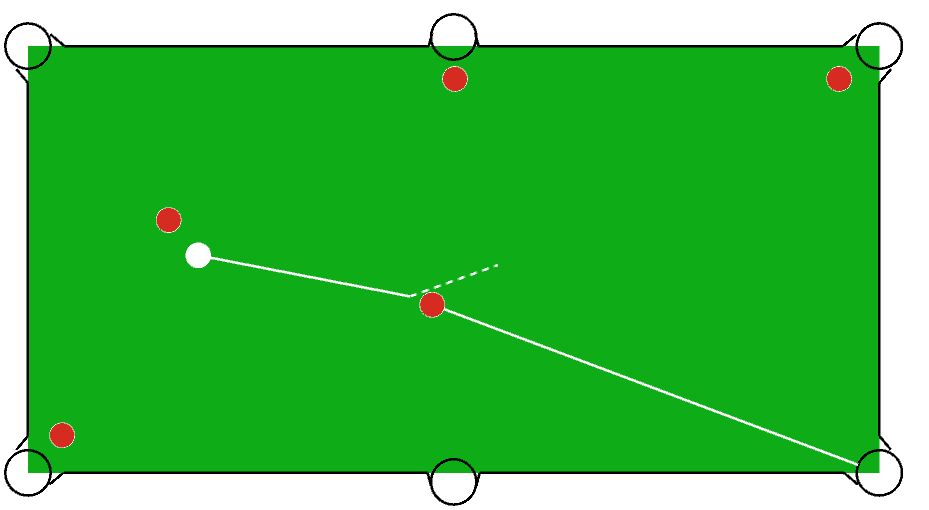
\includegraphics[width=1.0\linewidth]{../common/04_results/resources/simple_search/situation_diverse_solution_4.PNG}
        \caption{Stoss 4}
        \label{fig:situation_1_solution_4}
    \end{subfigure}
    \hfill
    \begin{subfigure}[b]{0.3\textwidth}
        \centering
        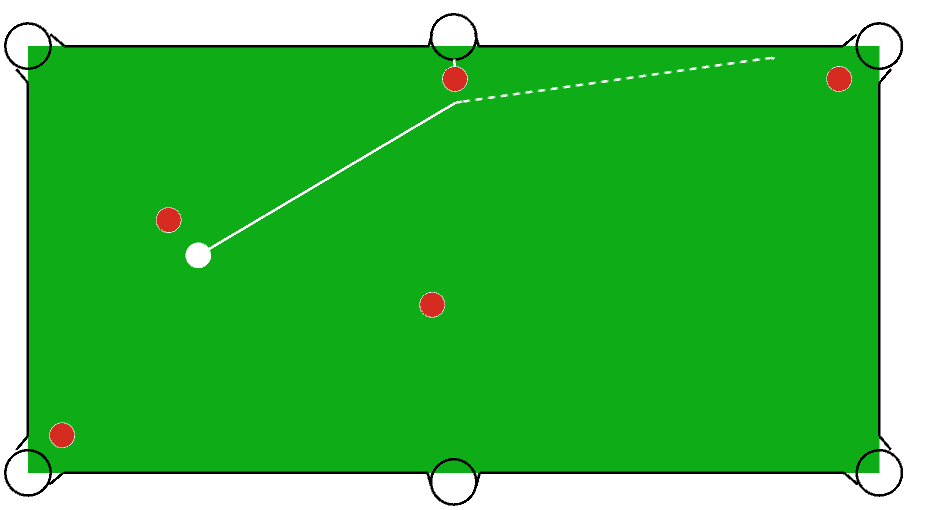
\includegraphics[width=1.0\linewidth]{../common/04_results/resources/simple_search/situation_diverse_solution_5.PNG}
        \caption{Stoss 5}
        \label{fig:situation_1_solution_5}
    \end{subfigure}
    \hfill
    \begin{subfigure}[b]{0.3\textwidth}
        \centering
        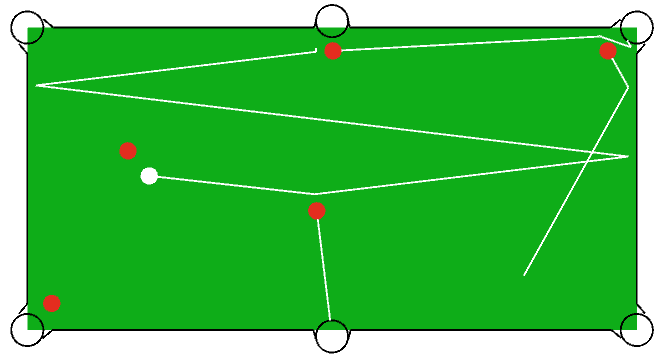
\includegraphics[width=1.0\linewidth]{../common/04_results/resources/simple_search/situation_diverse_solution_6.PNG}
        \caption{Stoss 6}
        \label{fig:situation_1_solution_6}
    \end{subfigure}
    \caption{Gefundene Stösse zu Situation 1 nach bewerteter Schwierigkeit aufsteigend}
    \label{fig:situation_1_solutions}
\end{figure}

% TODO: Stoss "Kugel 5 ins Loch unten-rechts." ist nicht in den obigen Abbildungen enthalten, trotzdem schreiben wir "Die zuvor beschriebenen denkbaren Stösse wurden tatsächlich gefunden."
Die Meisten der zuvor beschriebenen denkbaren Stösse wurden tatsächlich gefunden.
Der Stoss 1 wurde als der einfachste Stoss bewertet, weil die gesamte zurückzulegende Distanz klein ist,
der Pfad der beteiligten Kugeln insgesamt sehr geradlinig ist und weil die Kugel 1 sehr nahe am Loch unten-links liegt.
Der zweiteinfachste Stoss 2 zeigt eine grössere Distanz, welche der Spielball zurücklegen muss und daher erfordert
der Stoss auch eine höhere Startgeschwindigkeit des Spielballs wodurch dieser als schwieriger eingestuft wird als Stoss 1.
Dafür ist die Kugel 2 sehr nahe am Loch oben-rechts, wodurch die Kugel nicht mit absoluter Genauigkeit getroffen werden
muss, damit diese den erwünschten Pfad nicht so weit verlässt, dass sie das Ziel verfehlt.

Im Stoss 3 ist die Gesamtdistanz klein, allerdings ist die Distanz der Kugel 4 zum Spielball kleiner als die Distanz zum Loch.
Dadurch führt ein kleiner Fehler beim Treffen der Kugel zu einer grösseren Abweichung des Pfades.
In diesem Beispiel könnte dieser Fehler allerdings relativ klein sein, da der Pfad geradlinig ist und der Spielball die Kugel
nicht in einem Winkel treffen muss.

Stoss 2 wurde besser als Stoss 3 bewertet, weil bei Stoss 2 die Kugel näher am Loch liegt als bei Stoss 3. Die anderen
Bewertungskriterien Distanz und Winkel sind bei Stoss 3 besser als bei Stoss 2.
Ob diese Rangfolge objektiv korrekt ist, ist schwierig zu beurteilen.

Der Stoss 5 wird als schwieriger bewertet, weil der Winkel, in dem der Spielball die Kugel 3 treffen muss ca 45$^{\circ}$ ist.
Im Gegensatz dazu ist die Distanz der Kugel zum Loch sehr klein und die Gesamtdistanz ist relativ klein, was diesen Stoss
wiederum einfacher macht. Trotzdem hat in diesem Fall der Winkel die Bewertung so stark reduziert, dass Stoss 4 trotzdem
als einfacher eingestuft wird.

Stoss 6 zeigt die Idee, Kugel 5 ins Loch unten-zentral zu spielen.
Dazu muss diese in einem sehr grossen Winkel angespielt werden, was die Treffgenauigkeit reduziert und eine
erhöhte Startgeschwindigkeit des Spielballs erfordert.
Die weiteren weissen Linien zeigen den weiteren Verlauf der weissen Kugel, welche noch weitere Kugeln anstösst und
eine weitere rote Kugel ins Loch spielt, wodurch 2 Punkte statt einem Punkt gemacht werden.
Es wirkt unwahrscheinlich, dass die zweite rote Kugel tatsächlich ins Loch gespielt werden kann, da der Pfad der weissen Kugel
sehr lange ist und zwei Bandenkollisionen und zwei Kugelkollisionen enthält, bevor diese ins Loch rollt.
Allerdings sorgt der grosse Winkel, in dem die Kugel 5 angespielt werden muss dafür, dass dieser Stoss als sehr schwierig
bewertet wird, was den Nutzen von einem zusätzlichen Punkt überwiegt.

Aus den obigen Resultaten ist ersichtlich, dass die Suche diejenigen Stösse vorschlägt, welche nach Studium des Spielstandes
möglich erscheinen. Zudem berücksichtigt die Bewertung der Schwierigkeit eines Stosses die gesamte Distanz, die Winkel und die Nähe
der einzulochenden Kugel zum Loch.

% TODO: fall beschreiben, wo ein stoss nicht möglich ist, weil eine andere kugel im weg liegt

% TODO: resultate der suche indirekter stösse beschreiben, sofern umgesetzt

% TODO: resultate der suche über mehrere stösse beschreiben, sofern umgesetzt


% TODO: maybe describe, otherwise delete images
%
%State (for reproducing the results):
%WHITE0, WHITE, -0.925876, 9.06096
%RED1, RED, -0.925876, -345.584
%RED2, RED, -0.925876, 246.79
%

%\begin{figure}[h!]
%    \begin{center}
%        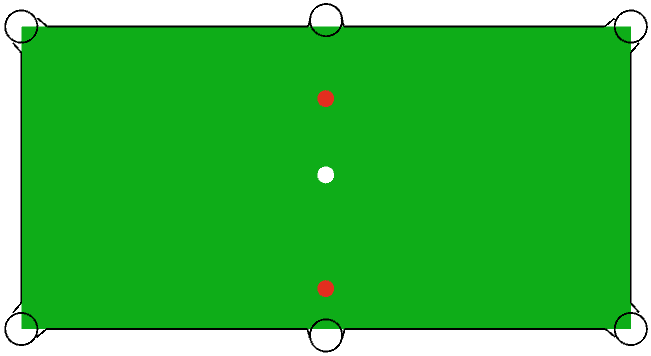
\includegraphics[width=0.4\linewidth]{../common/04_results/resources/simple_search/situation_similar_distance_but_one_is_closer_to_pocket.PNG}
%    \end{center}
%    \caption{Situation 2: Eine Kugel ist näher am Ziel als eine andere}
%    \label{fig:search_situation_2}
%\end{figure}

%\begin{figure}
%    \centering
%    \begin{subfigure}[b]{0.4\textwidth}
%        \centering
%        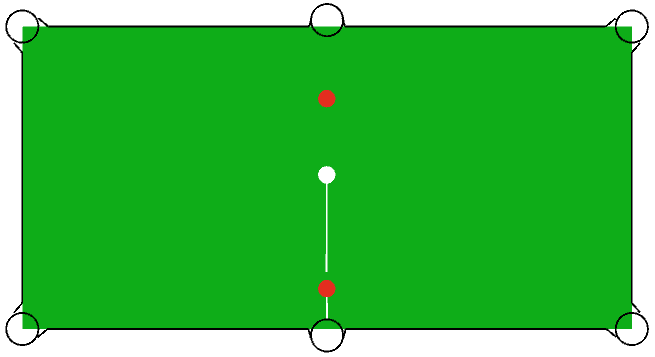
\includegraphics[width=1.0\linewidth]{../common/04_results/resources/simple_search/situation_similar_distance_but_one_is_closer_to_pocket_solution_1.PNG}
%        \caption{Stoss 1}
%        \label{fig:situation_2_solution_1}
%    \end{subfigure}
%    \hfill
%    \begin{subfigure}[b]{0.4\textwidth}
%        \centering
%        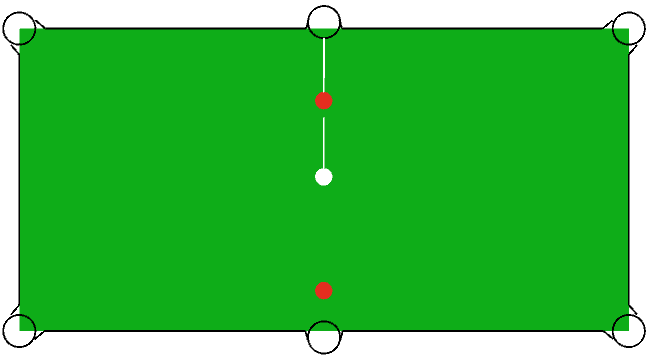
\includegraphics[width=1.0\linewidth]{../common/04_results/resources/simple_search/situation_similar_distance_but_one_is_closer_to_pocket_solution_2.PNG}
%        \caption{Stoss 2}
%        \label{fig:situation_2_solution_2}
%    \end{subfigure}
%    \caption{Gefundene Stösse zu Situation 2 nach bewerteter Schwierigkeit aufsteigend}
%    \label{fig:situation_2_solutions}
%\end{figure}

% TODO: maybe describe, otherwise delete images
%
%State (for reproducing the results):
%WHITE0, WHITE, 14.5049, 9.06096
%RED1, RED, -598.867, -146.827
%RED2, RED, 492.858, -240.359
%
%\begin{figure}[h!]
%    \begin{center}
%        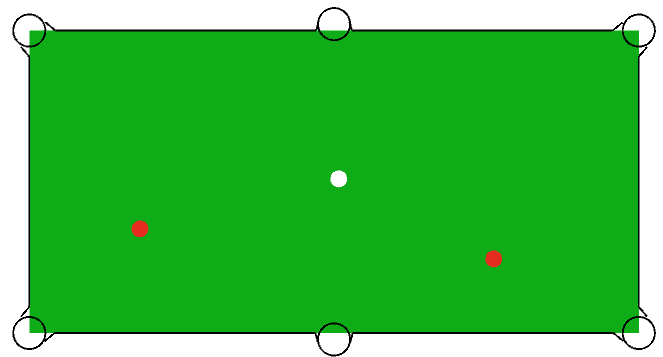
\includegraphics[width=0.4\linewidth]{../common/04_results/resources/simple_search/situation_similar_distance_different_angles.PNG}
%    \end{center}
%    \caption{Situation 3: Eine Kugel muss in einem grösseren Winkel angespielt werden als die andere.}
%    \label{fig:search_situation_3}
%\end{figure}

%\begin{figure}
%    \centering
%    \begin{subfigure}[b]{0.4\textwidth}
%        \centering
%        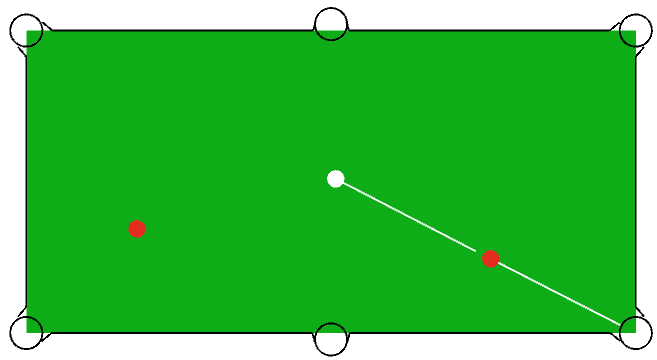
\includegraphics[width=1.0\linewidth]{../common/04_results/resources/simple_search/situation_similar_distance_different_angles_solution_1.PNG}
%        \caption{Stoss 1}
%        \label{fig:situation_3_solution_1}
%    \end{subfigure}
%    \hfill
%    \begin{subfigure}[b]{0.4\textwidth}
%        \centering
%        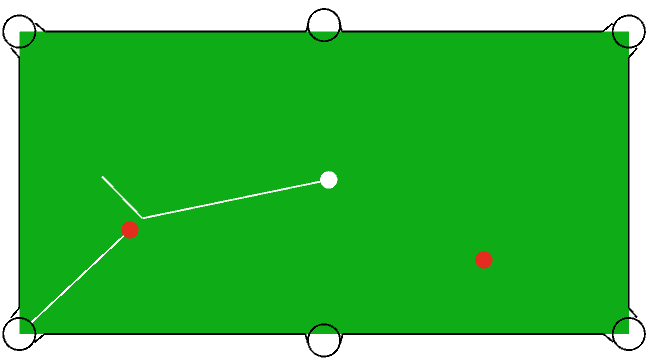
\includegraphics[width=1.0\linewidth]{../common/04_results/resources/simple_search/situation_similar_distance_different_angles_solution_2.PNG}
%        \caption{Stoss 2}
%        \label{fig:situation_3_solution_2}
%    \end{subfigure}
%    \caption{Gefundene Stösse zu Situation 3 nach bewerteter Schwierigkeit aufsteigend}
%    \label{fig:situation_3_solutions}
%\end{figure}

